\chapter{Metriche}

In questo capitolo verranno descritte le metriche anticipate nella Sezione
\ref{descrizione_progetto}, mostrando il relativo codice e i risultati ottenuti.

\section{Metriche sulle conferenze}

Questa sezione tratta delle varie metriche relative all'insieme di conferenze
analizzate, che conta un totale di più di 500 conferenze.

\subsection{Rating delle conferenze}

Come descritto in Sezione~\ref{sec:conferenze}, le conferenze possono avere
un rating, rappresentato da una lettera, che rappresenta la qualità generale
della conferenza.

Al fine di comprendere al meglio come questa classifica influenza i vari indici
bibliometrici, in Figura~\ref{fig:conferences-distribution} viene rappresentata
la suddivisione delle conferenze in base alla loro qualità come classificata
dal GGS.

\begin{figure}[tb]
  \centering
  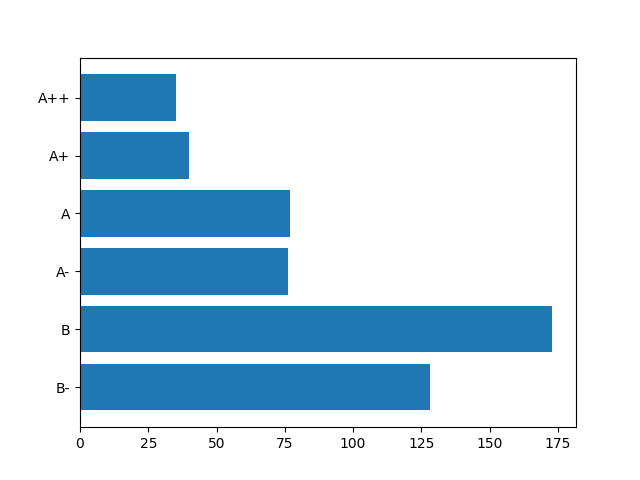
\includegraphics[width=\linewidth]{conferences-distribution.png}
  \caption{Distribuzione delle conferenze}
  \label{fig:conferences-distribution}
\end{figure}

È immediato notare che la distribuzione è suddivisa in 3 gruppi principali:
\begin{enumerate}
  \item Il gruppo delle ``conferenze top'', dato dalle A++ e dalle A+, che
        risulta essere il più contenuto di tutti con meno di 100 conferenze;
  \item Il secondo gruppo delle conferenze di alto livello, dato dalle A e A-,
        che risulta comunque non molto più grande del precedente con circa 150
        conferenze;
  \item Ed infine il gruppo delle conferenze B e B-, che domina in quanto a numero
        i precedenti due, avendo più conferenze degli altri due gruppi combinati.
\end{enumerate}

Questo conferma quello che ci si può aspettare con la classificazione per qualità in molti ambiti: in generale, la qualità alta è correlata
con una numerosità minore.

Ciò fa sì che conferenze con qualità più alta, essendo in numero minore,
ricevano una competizione maggiore rispetto a quelle di qualità più bassa, in
quanto una conferenza di ottimo livello tenderà ad essere più critica sui lavori
ricevuti al fine di mantenere tale ranking. D'altra parte, una conferenza con
ranking minore potrebbe puntare maggiormente sulla quantità di paper al fine di
crescere di dimensioni per poter avere una possibilità di salire di ranking,
ma a scapito del controllo della qualità dei lavori ad essa sottomessi. Questo infatti è uno dei criteri considerati dal CORE per la valutazione della qualità di una conferenza (come approfondito nella Sezione \ref{sec:conferenze_scientifiche}).

\subsection{Numero di citazioni per paper in base al rating}

Si vuole ora guardare a come la qualità di una conferenza influenza il numero
di citazioni che un paper prende in media. Il numero di citazioni di un paper
è una metrica importante per un ricercatore, in quanto è uno dei fattori
che contribuisce ai suoi indici principali, tra cui l'$h$-index.

La Figura~\ref{fig:paper-rating-distribution} mostra appunto tale distribuzione,
rappresentando con un punto il numero di citazioni di ogni singolo paper e
con una linea rossa la media di citazioni in base al rating della conferenza
a cui il paper è stato sottomesso. I valori di tale media sono visibili
anche in Tabella~\ref{table:paper-rating-distribution}.

\begin{figure}[tb]
  \centering
  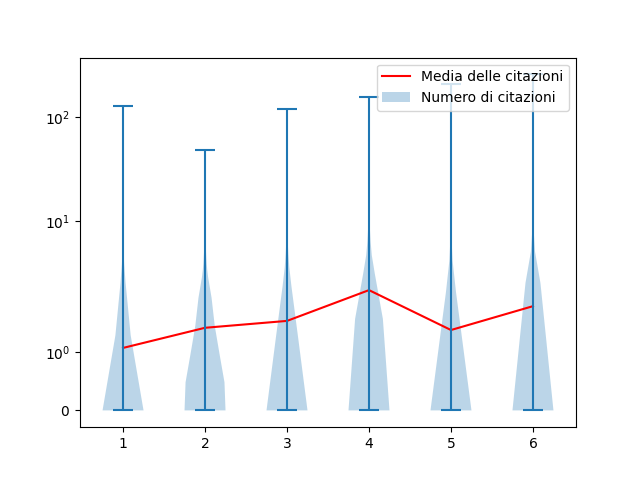
\includegraphics[width=\linewidth]{paper_rating_distribution.png}
  \caption{Numero di citazioni per conferenza}
  \label{fig:paper-rating-distribution}
\end{figure}

\begin{figure}[tb]
  \centering
  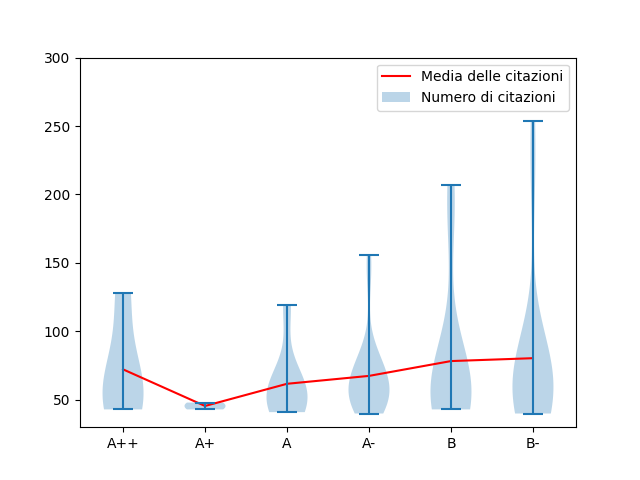
\includegraphics[width=\linewidth]{paper_rating_distribution_impact.png}
  \caption{Numero di citazioni di paper di impatto per conferenza}
  \label{fig:paper-rating-distribution-impact}
\end{figure}

\begin{table}[tb]
  \centering
  \begin{tabular}{||l | r | r ||}
    \hline
    \multirow{2}{*}{\textbf{Rating}} & \multicolumn{2}{| c ||}{\textbf{Numero di citazioni medio}} \\ \cline{2-3}
     & \textbf{Tutti i paper} & \textbf{Paper di impatto} \\ [0.5ex] 
    \hline\hline
    A++    & 1.08 & 72.25 \\ \hline
    A+     & 1.42 & 45.50 \\ \hline
    A      & 1.54 & 61.71 \\ \hline
    A-     & 2.19 & 67.48 \\ \hline
    B      & 1.38 & 78.32 \\ \hline
    B-     & 1.80 & 80.41 \\ \hline
  \end{tabular}
  \caption{Numero di citazioni medio per rating}
  \label{table:paper-rating-distribution}
\end{table}

Dall'immagine è possibile trarre due conclusioni importanti:
\begin{enumerate}
  \item La prima è che, in media, le citazioni per un paper sono basse sul
        periodo di qualche anno che è stato considerato;
  \item La seconda, invece, è che la distribuzione delle citazioni è molto sbilanciata,
        in quanto ci sono molti paper con poche citazioni e pochi paper che superano
        le 40 citazioni.
\end{enumerate}

Queste due conclusioni valgono inoltre per qualsiasi ranking di conferenza,
con un leggero aumento per le conferenze di livello inferiore.
Si può quindi dedurre che, in genere, il livello di una conferenza non influenza
il numero di citazioni ottenute nel breve periodo, con anzi
un aumento delle citazioni in media per conferenze non top, ovvero con ranking
da A in giù.

Può essere interessante inoltre guardare ai paper che possiamo definire come
``d'impatto'', ovvero i pochi paper che superano le 40 citazioni identificati
dalle conclusioni precedenti. Tale distribuzione è visibile in
Figura~\ref{fig:paper-rating-distribution-impact} e, similmente a prima,
è possibile vedere i numeri precisi in
Tabella~\ref{table:paper-rating-distribution}.
Guardando il grafico, è possibile notare che i paper con citazioni più alte
si trovano sulle conferenze di rating più basso, ma questi risultano essere più
valori rari che si discostano molto dalla media. Sulle conferenze di livello
più alto, invece, la distribuzione è molto meno sbilanciata: i paper sono più
concentrati sotto le 150 citazioni, ma in genere la distribuzione di citazioni
è più equa. Questo si vede chiaramente per le conferenze A++.

\subsection{Media dell'$h$-index per conferenza in base al rating}

Oltre al numero di citazioni, è interessante guardare anche
a come l'$h$-index degli autori è correlato con il rating delle conferenze
a cui partecipano. Questo perché ci si aspetta che conferenze con un rating
maggiore attirino ricercatori con più esperienza, in quanto il loro
processo di accettazione è sicuramente più selettivo rispetto a conferenze
più nuove oppure semplicemente classificate come di livello inferiore.

Nella Figura~\ref{fig:h-index-vs-rating} si vede appunto questa metrica,
rappresentata tramite un grafico a violino con in rosso la media dell'$h$-index
per rating della conferenza, i cui valori precisi sono visibili in
Tabella~\ref{table:h-index-vs-rating}.

\begin{figure}[tb]
  \centering
  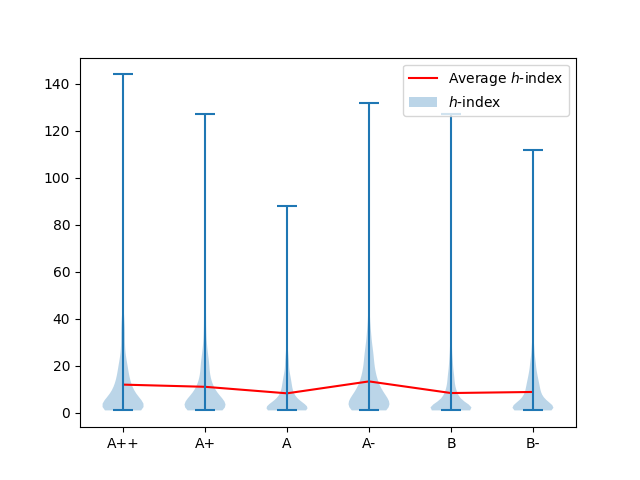
\includegraphics[width=\linewidth]{h_index_vs_conference_rating.png}
  \caption{$h$-index per conferenza}
  \label{fig:h-index-vs-rating}
\end{figure}

\begin{table}[tb]
  \centering
  \begin{tabular}{||l|r||}
    \hline
    \textbf{Rating conferenza} & \textbf{$h$-index medio} \\ [0.5ex] 
    \hline\hline
    A++    & 11.97 \\ \hline
    A+     & 11.04 \\ \hline
    A      & 8.27  \\ \hline
    A-     & 13.34 \\ \hline
    B      & 8.39 \\ \hline
    B-     & 8.84 \\ \hline
  \end{tabular}
  \caption{Valori medi dell'$h$-index}
  \label{table:h-index-vs-rating}
\end{table}

Come si può vedere dai dati, per le conferenze di livello ottimo (A++ e A+)
si ha un $h$-index maggiore in media, pari a circa $11.51$, rispetto a quelle
degli altri due livelli ($10.81$ per le conferenze A e A-, $8.62$ per le B e
B-).

Questo coincide con le aspettative: conferenze di livello maggiore hanno
un processo selettivo più restrittivo e di conseguenza è più probabile
che un ricercatore con più esperienza (e quindi con $h$-index probabilmente
più alto) sottoponga lavori a queste conferenze.

Notare comunque che la differenza fra le varie categorie non è così elevata,
e le curve sono fortemente sbilanciate verso $h$-index bassi in ogni caso,
anche se ciò è più visibile nelle conferenze di rating B e B-.

\section{Metriche sulle affiliazioni}

Questa sezione tratta di alcune metriche per le affiliazioni, in particolare
raggruppate per stato di appartenenza. Ciò al fine di capire al meglio
in che aree e in che realtà si concentra la ricerca in ambito informatico.

Il numero di affiliazioni considerate conta poco meno di 13000 fra università
e centri di ricerca, con un totale di 131 nazioni.

\subsection{Autori e documenti per stato di appartenenza}
\label{ssec:authors-docs-per-country}

Tale metrica viene analizzata principalmente come base per le successive, in
quanto uno stato con molti più autori ha anche molta più probabilità di avere
università considerate migliori, il che potrebbe portare ad un aumento
in generale dell'$h$-index medio o della qualità della ricerca.
Tale numero è visibile, per le prime 10 nazioni in ordine di numero di autori,
in Figura~\ref{fig:num-authors-per-country}.

Inoltre, sono stati anche calcolati il numero di documenti prodotti dalle singole
nazioni, per ragioni simili a quelle esplicate nel paragrafo precedente: un
paese con molti più documenti rappresenta una maggiore concentrazione della
ricerca, che potrebbe essere correlata con maggiore qualità.
Tale metrica è visibile in Figura~\ref{fig:num-documents-per-country}.

\begin{figure}[tb]
  \centering
  \begin{subfigure}[b]{0.45\textwidth}
    \centering
    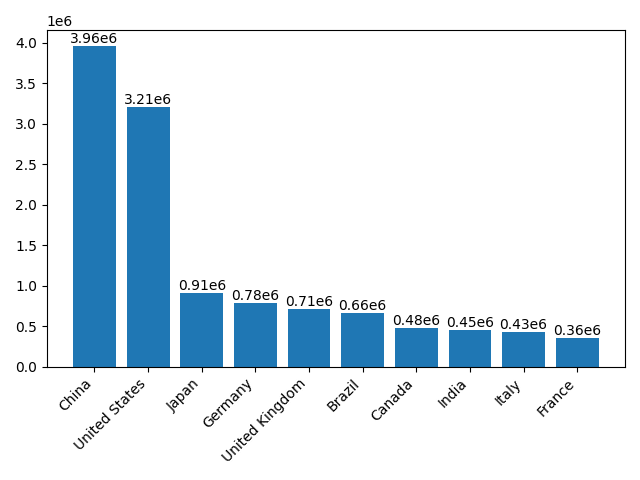
\includegraphics[width=\textwidth]{num_authors_per_country.png}
    \caption{Numero di autori}
    \label{fig:num-authors-per-country}
  \end{subfigure}
  \begin{subfigure}[b]{0.45\textwidth}
    \centering
    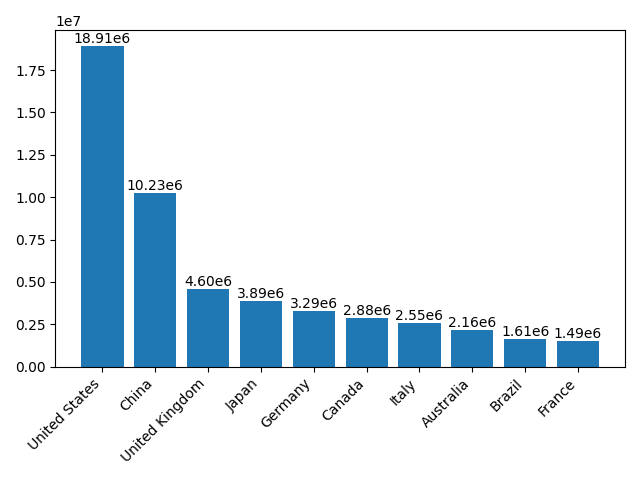
\includegraphics[width=\textwidth]{num_documents_per_country.png}
    \caption{Numero di documenti}
    \label{fig:num-documents-per-country}
  \end{subfigure}
  \caption{Primi 10 stati secondo varie metriche}
  \label{fig:top-10-country}
\end{figure}

Non sorprendentemente, i dati raccolti confermano che gli attuali stati
con più ricercatori in ambito di computer science sono la Cina e gli Stati Uniti,
dopo i quali il numero di autori diventa meno di un terzo per altri paesi
dell'Asia, dell'Europa e del Nord America.
Per quanto riguarda i documenti, invece, gli Stati Uniti dominano, ma sono
seguiti a breve distanza dalla Cina.

Di conseguenza, ci si aspetta che la Cina e gli Stati Uniti tengano delle buone
posizioni nelle successive classifiche, in quanto dispongono di un parco maggiore
di ricercatori e producono un maggiore numero di documenti.

Interessante notare l'Italia che si pone come terza nazione europea per numero
di autori, dietro a Germania e Regno Unito, in entrambi i casi.

\subsection{Maggiori entità per produttività}

In genere guardare al solo numero assoluto di autori o documenti di un certo
stato è sì interessante, ma lontano dal quadro completo. Per questo si è
deciso di introdurre un'ulteriore metrica, qui chiamata \textit{produttività},
definita semplicemente come il rapporto fra il numero di documenti ed il
numero di autori. In tal modo, un valore alto di produttività indica uno
stato in cui i ricercatori producono in media più lavori rispetto ad un
altro. Nella Figura~\ref{fig:productivity-per-country} vengono quindi mostrati i valori
di produttività calcolati sugli stati con maggiore numero di autori e di
documenti, ovvero gli stati visibili in Figura~\ref{fig:top-10-country} alla
Sezione~\ref{ssec:authors-docs-per-country}.

\begin{figure}[tb]
  \centering
  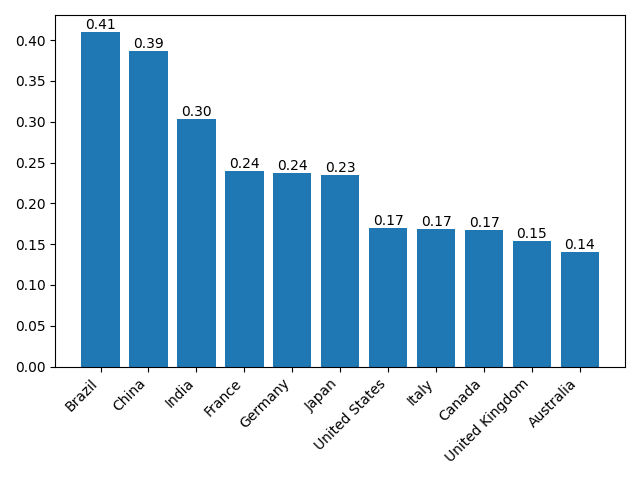
\includegraphics[width=\linewidth]{productivity_per_country.png}
  \caption{Produttività per le maggiori nazioni}
  \label{fig:productivity-per-country}
\end{figure}

Dalla figura compare uno scenario leggermente diverso: le maggiori nazioni
per produttività non sono le maggiori per numero di documenti o autori, eccezion
fatta per la Cina. La produttività maggiore va invece verso nazioni come Brasile
e India, subito seguite da Francia e Germania.
Di conseguenza, i paesi in cui i ricercatori producono più lavori in media
sono i paesi cosiddetti ``emergenti''.
\todo{Capire se questa frase è da sistemare}

\section{Metriche sugli autori}

% \chapter{Metriche}
%In questo capitolo verranno descritte le metriche anticipate nella Sezione \ref{descrizione_progetto}, mostrando il relativo codice e i risultati ottenuti.

%\section{Distribuzione della qualità delle conferenze}


%\section{Distribuzione degli H-index degli autori}
%\section{Distribuzione della qualità dei lavori per autore}
%\section{Correlazione tra qualità delle conferenze e numero di citazioni del paper}
%\section{Correlazione tra qualità della conferenza e distribuzione degli H-index degli autori coinvolti}